\documentclass[11pt]{article}

% Packages
\usepackage[margin=1in]{geometry}
\usepackage{amsmath}
\usepackage{amssymb}
\usepackage{graphicx}
\usepackage{float}
\usepackage{booktabs}
\usepackage{enumitem}

\title{Homework 4}
\author{Fhaheem Tadamarry}
\date{\today}

\begin{document}

\maketitle

\section*{Instruction-Level, Data-Level, and Thread-Level Parallelism}

\begin{enumerate}

    \item \textbf{Vector Processing - Basic Idea (15 pts)} \\
    A \textbf{vector processor} operates on entire arrays of data (vectors) with a single instruction, exploiting data-level parallelism (DLP). This contrasts with scalar processors that operate on one data element at a time. Vector processors use pipelined functional units to execute operations across vector elements efficiently.

    \textbf{Key Features:}
    \begin{itemize}
        \item SIMD architecture (Single Instruction, Multiple Data).
        \item Supports vector registers and vector instructions.
        \item High throughput due to overlapping execution (pipelining).
        \item Reduces instruction-fetch overhead and loop control complexity.
    \end{itemize}

    \item \textbf{RISC-V Vector Architecture Block Diagram (20 pts)} \\
    \begin{center}
        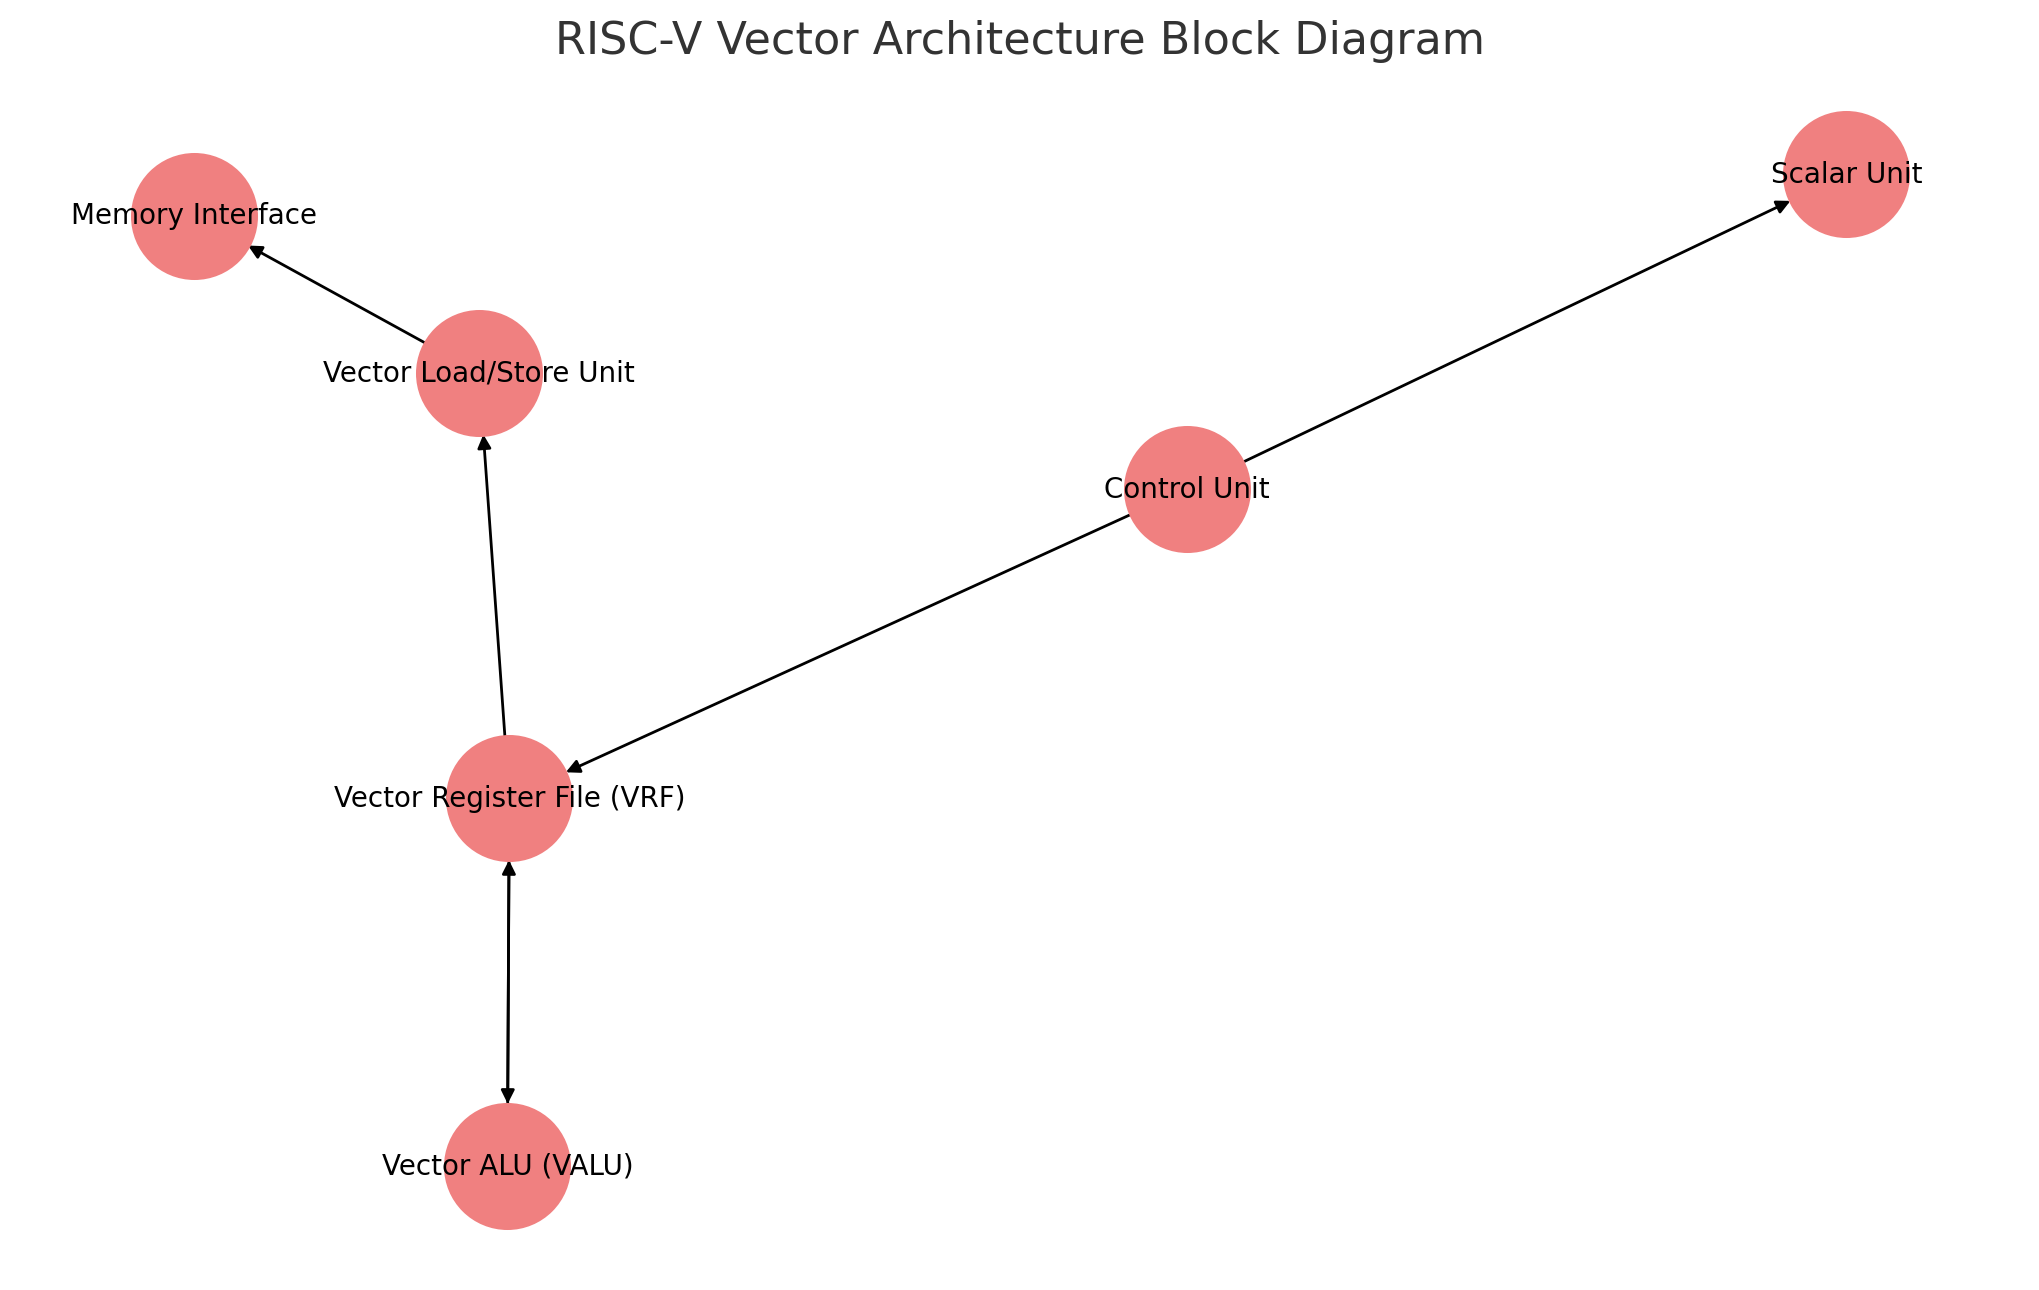
\includegraphics[width=0.8\textwidth]{RISC-V Vector Architecture Block Diagram.png}
    \end{center}

    \textbf{Explanation of Blocks:}
    \begin{itemize}
        \item \textbf{Vector Register File (VRF):} Holds vector operands and results.
        \item \textbf{Vector Arithmetic Logic Unit (VALU):} Executes vector arithmetic and logic operations.
        \item \textbf{Vector Load/Store Unit:} Manages data transfer between memory and VRF.
        \item \textbf{Scalar Unit:} Handles scalar operations.
        \item \textbf{Control Unit:} Decodes vector instructions, controls the pipeline, and manages vector length.
        \item \textbf{Memory Interface:} Connects to main memory for vector element access.
    \end{itemize}

    \item \textbf{Vector Processing Techniques (20 pts)} \\
    \begin{enumerate}[label=\alph*.]
        \item \textbf{Vector Chaining:} \\
        Allows vector functional units to start executing a new operation before the previous one finishes. The output of one operation can directly feed into the next, reducing pipeline latency.
        \\ \textit{Example:} Multiply a vector by a scalar and then add another vector without waiting for the full multiplication to complete.

        \item \textbf{Strip Mining:} \\
        Breaks down vector operations into smaller chunks when the vector length exceeds the hardware vector length. Useful for handling loops where data size is larger than the available vector registers.
        \\ \textit{Example:} If hardware supports vectors of length 64 but data size is 200, the operation is broken into four chunks (64, 64, 64, and 8).

        \item \textbf{Vector Stride:} \\
        Specifies the step between elements in memory for vector operations. Used for accessing non-contiguous memory locations.
        \\ \textit{Example:} Access every 3rd element in an array: stride = 3.

        \item \textbf{Gather and Scatter:} \\
        - \textbf{Gather:} Loads elements from non-contiguous memory addresses into a vector register based on an index array. \\
        - \textbf{Scatter:} Stores elements from a vector register to non-contiguous memory addresses using an index array. \\
        Useful for irregular data structures like sparse matrices.
    \end{enumerate}

    \item \textbf{Snooping Protocol - Problem 5.1 (20 pts)} \\
    \begin{enumerate}[label=\alph*.]
        \item \textbf{What are the four states of the MSI protocol?} \\
        The four states of the MSI protocol are:
        \begin{itemize}
            \item \textbf{M (Modified):} The cache block is modified and is the only valid copy.
            \item \textbf{S (Shared):} The cache block is clean and may be shared among other caches.
            \item \textbf{I (Invalid):} The cache block is invalid.
            \item \textbf{Exclusive (sometimes included in MESI variant, not pure MSI):} Only in MESI, not MSI.
        \end{itemize}

        \item \textbf{What happens on a processor read hit and miss?} \\
        \textbf{Read Hit:} Data is read from the cache without generating any coherence traffic. \\
        \textbf{Read Miss:} The cache issues a BusRd (bus read) transaction. Other caches may respond with their shared data. If no cache responds, data is fetched from memory. The cache enters the \textbf{Shared} state after the miss.

        \item \textbf{What happens on a processor write hit and miss?} \\
        \textbf{Write Hit:}
        \begin{itemize}
            \item If in \textbf{Modified} state: Directly update the cache.
            \item If in \textbf{Shared} state: Issue BusUpgr (bus upgrade) to invalidate other shared copies and transition to \textbf{Modified}.
        \end{itemize}
        \textbf{Write Miss:} Issues BusRdX (bus read exclusive) to fetch data and invalidate copies in other caches. The cache then transitions to the \textbf{Modified} state.
    \end{enumerate}

    \item \textbf{Coherence Protocols Explanation (15 pts)} \\
    \begin{enumerate}[label=\alph*.]
        \item \textbf{Snooping Coherence Protocol:} \\
        In snooping-based coherence, all caches monitor (snoop) the shared bus to determine if they need to take action on memory operations performed by other caches. If one cache writes to a shared block, all other caches snoop this transaction and invalidate their copies if required.
        \\ \textit{Example:} MSI and MESI protocols use snooping mechanisms.

        \item \textbf{Directory-Based Coherence Protocol:} \\
        Maintains a directory at the home node (associated with each memory block) to keep track of which caches have a copy of the block. Instead of broadcasting to all processors, the home node communicates only with the caches that hold the data, reducing unnecessary traffic.
        \\ \textit{Example:} Scales better than snooping for large multiprocessors since it avoids global broadcasts.
    \end{enumerate}

    \item \textbf{Directory Protocol with State Diagram (10 pts)} \\
    \textbf{(a) Read Miss Handling:} \\
    \begin{center}
        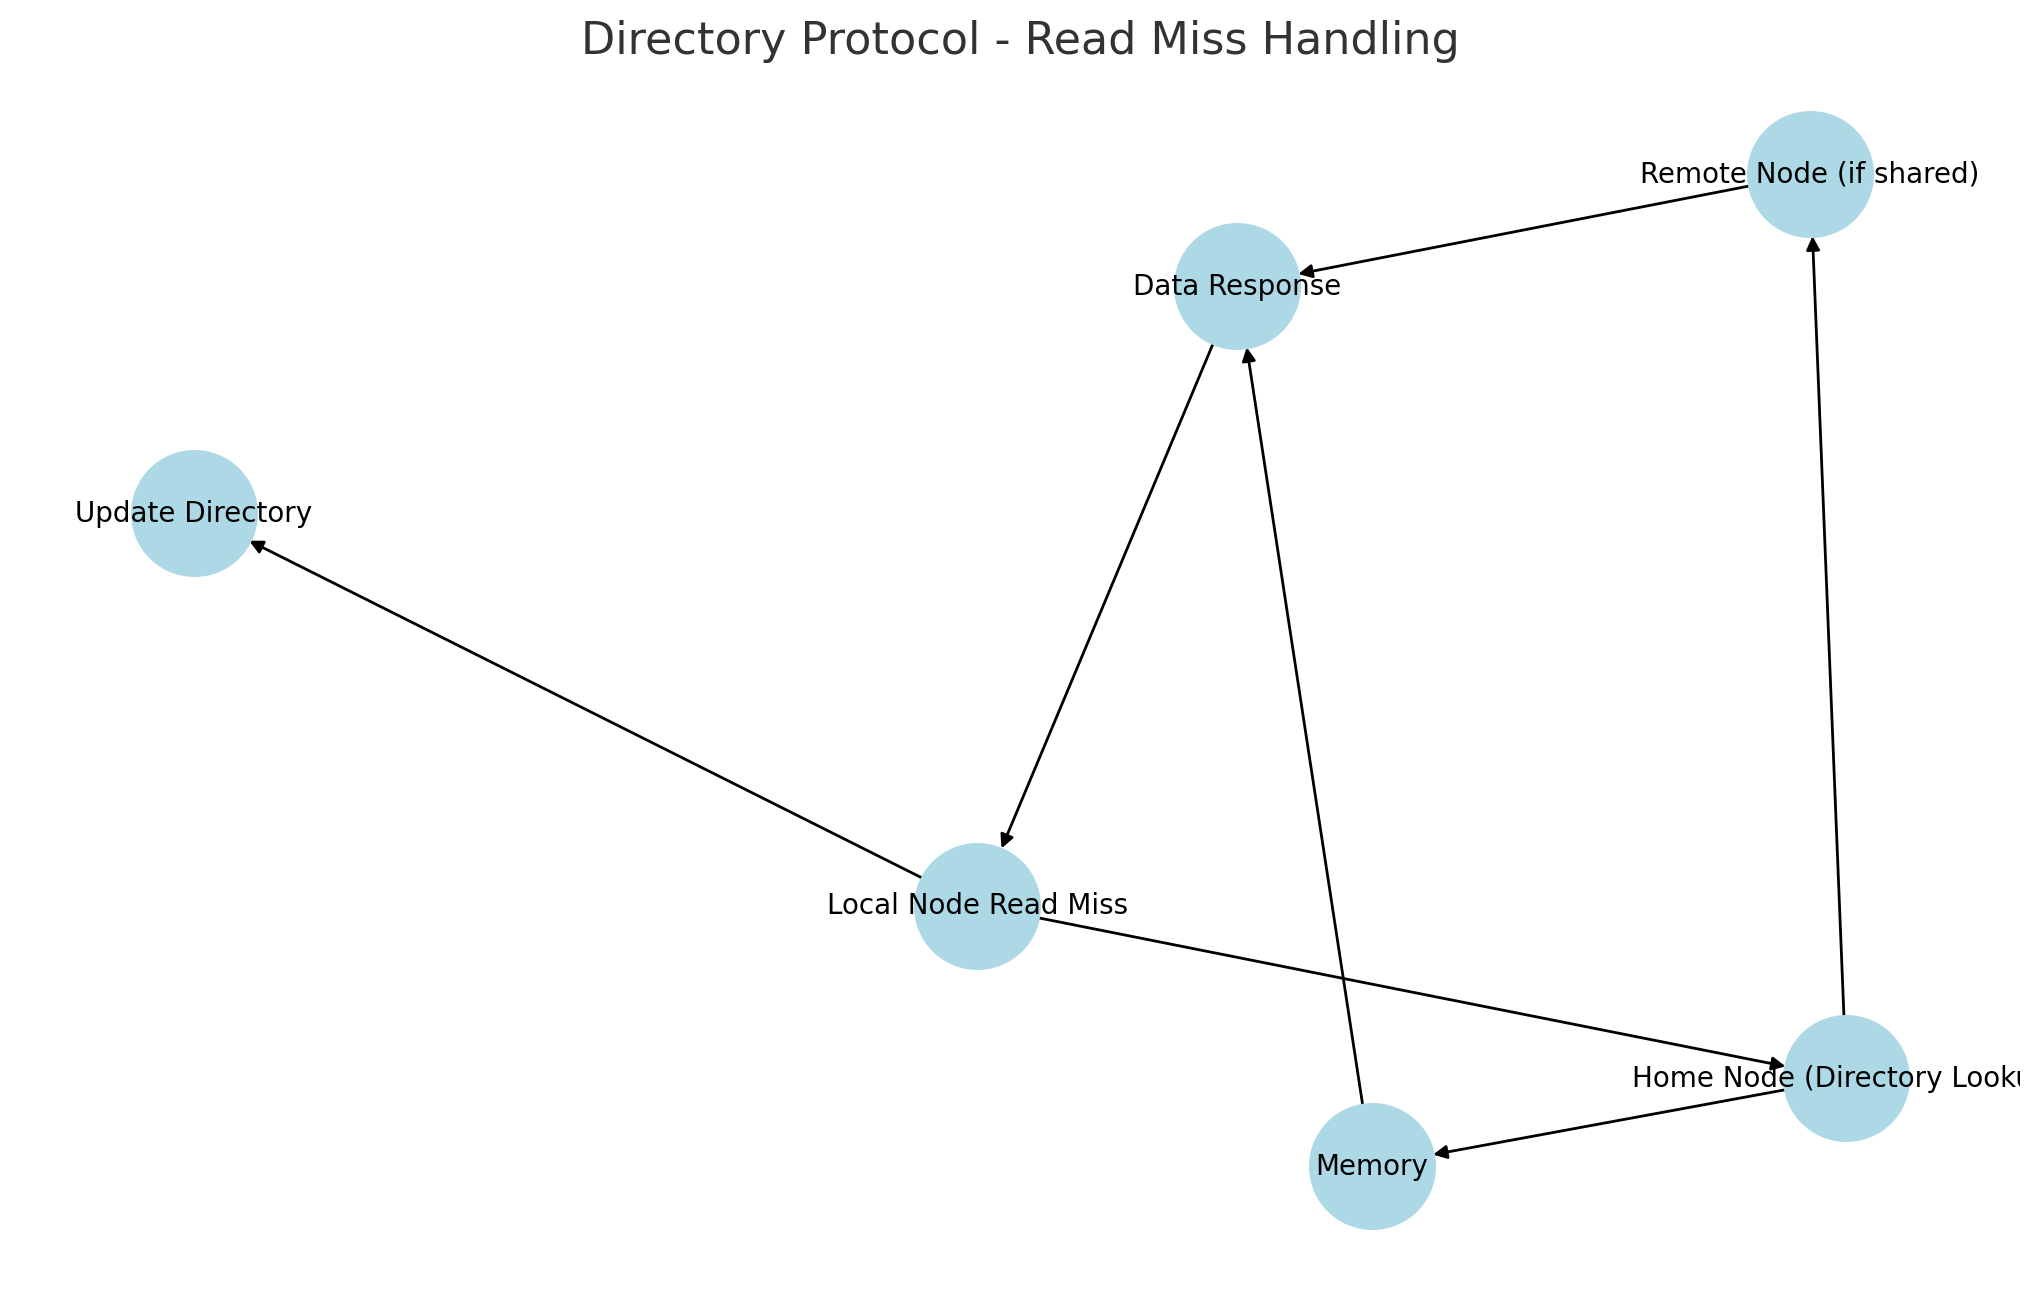
\includegraphics[width=0.7\textwidth]{Directory Protocol - Read Miss Handling.png}
    \end{center}
    \textbf{Explanation:}
    \begin{itemize}
        \item A read miss from a local node triggers a request to the home node.
        \item The home node checks the directory:
        \begin{itemize}
            \item If the block is not present in any cache, data is fetched from memory.
            \item If the block is present in other caches, the data is supplied from one of the remote nodes (if applicable).
        \end{itemize}
        \item The requesting node is added to the sharing set in the directory.
    \end{itemize}

    \textbf{(b) Write Miss Handling:} \\
    \begin{center}
        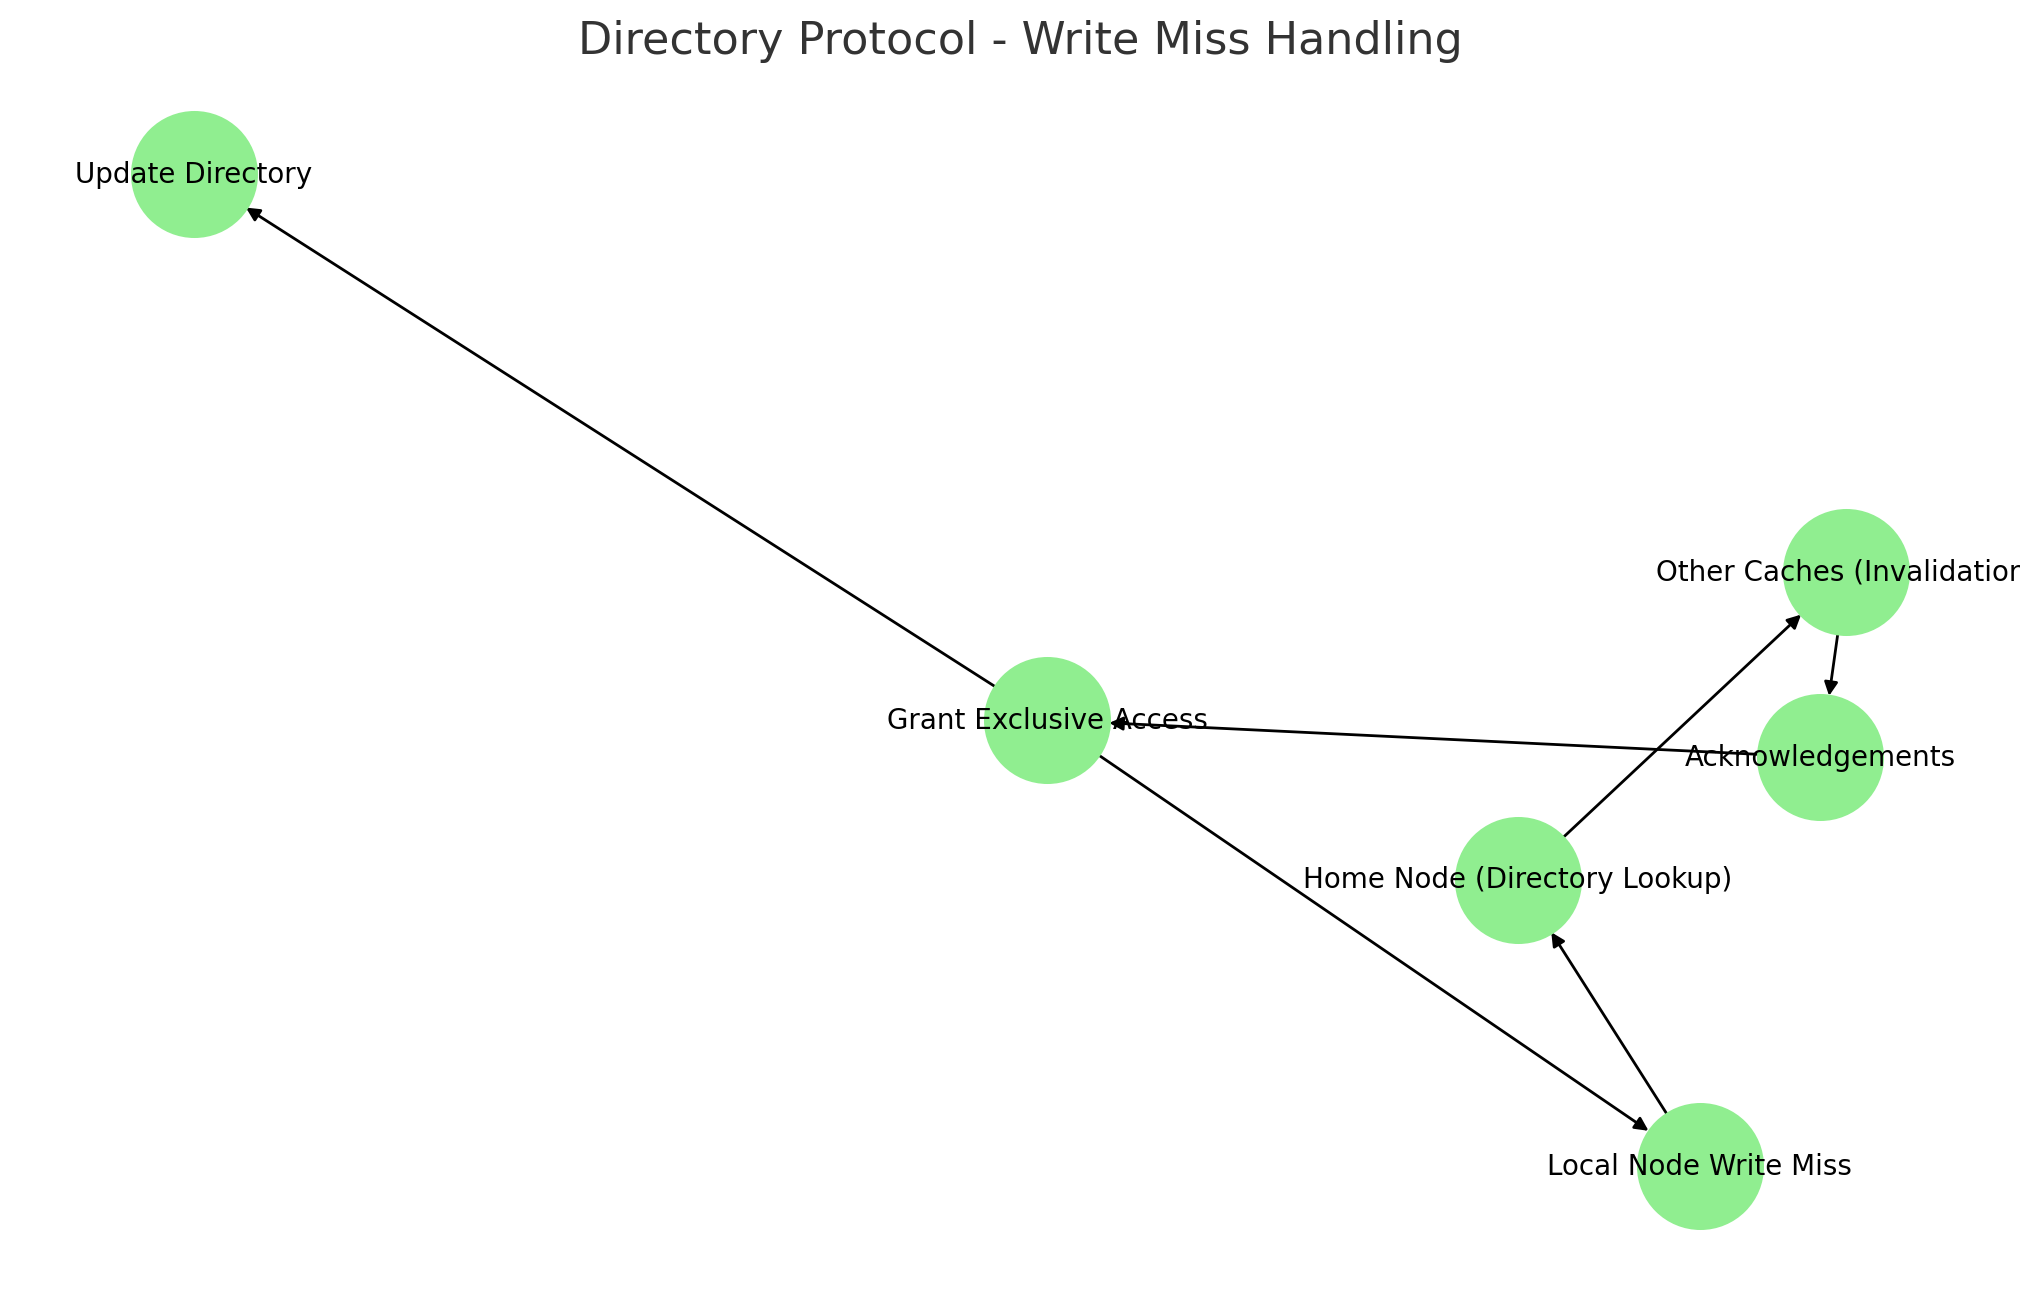
\includegraphics[width=0.7\textwidth]{Directory Protocol - Write Miss Handling.png}
    \end{center}
    \textbf{Explanation:}
    \begin{itemize}
        \item A write miss from a local node triggers a request to the home node.
        \item The home node sends invalidation messages to all nodes in the sharing set.
        \item Once invalidations are acknowledged, the home node grants exclusive access to the requesting node.
        \item The directory updates the owner to the requesting node, clearing the sharing set.
    \end{itemize}

\end{enumerate}

\end{document}
